\section{First start of the \emph{Reprotool IDE}}
When you run \emph{Reprotool} for the first time, the \emph{Reprotool} welcome page will be displayed. It is a hypertext page that
provides basic information about \emph{Reprotool}, a short 5-minutes tutorial and a link to further web resources about \emph{Reprotool}.

\begin{figure}[ht]
  \centering
  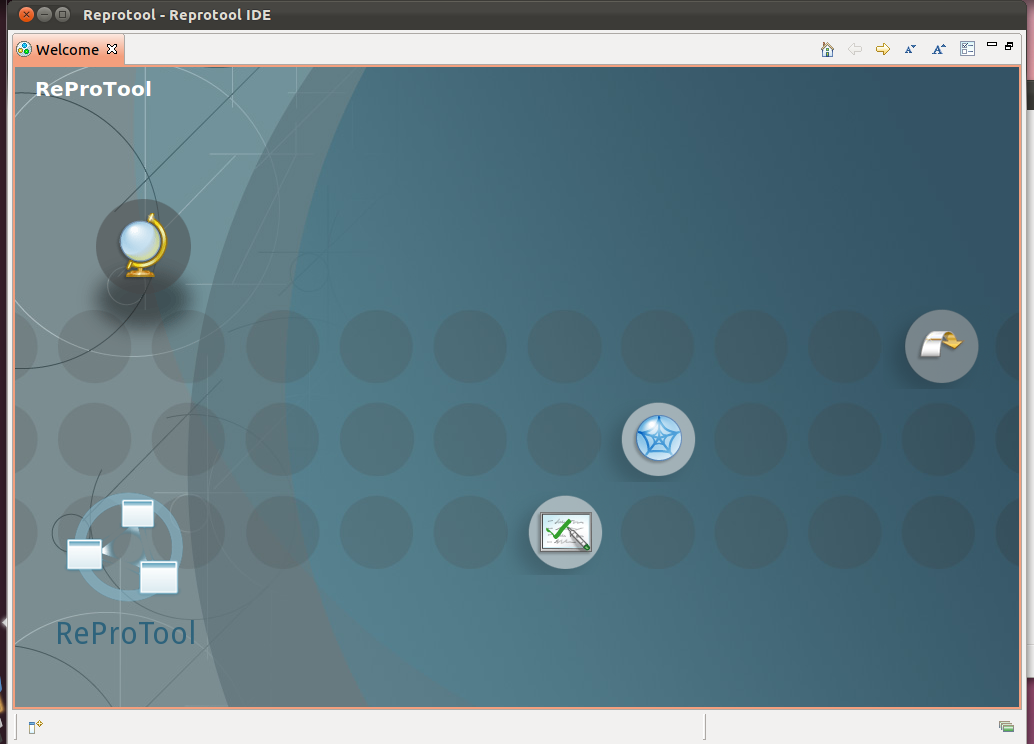
\includegraphics[height=280pt]{images/reprotoolWelcome}
  \caption{The \emph{Reprotool} welcome page}
  \label{fig:reprotoolWelcome}
\end{figure}

The \emph{tutorials} section contains a quick five-minutes tutorial that serves as an introduction to some of the \emph{Reprotool}
features. If you decide to skip this tutorial, you should at least install the \emph{Reprotool example projects} into your workspace
because you will need them in later parts of this documentation. Read the tutorial for information how to install the example projects.

If you display the \emph{Welcome page} in other that maximized mode, you will see the quick tutorial in the welcome page. This way, you
can easily follow the tutorial and perform the required steps in the workbench.

\begin{figure}[ht]
  \centering
  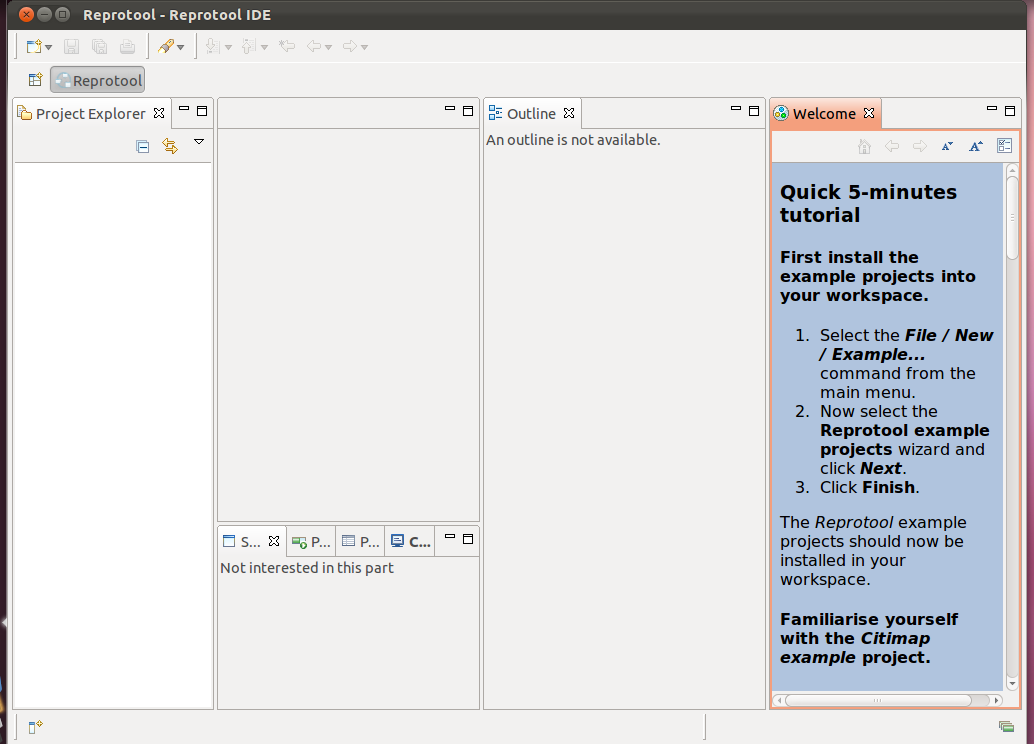
\includegraphics[height=280pt]{images/reprotoolWelcomeTutorial}
  \caption{The \emph{Reprotool} welcome page - quick tutorial}
  \label{fig:reprotoolWelcomeTutorial}
\end{figure}